\UseRawInputEncoding
\documentclass{article}

% Language setting
\usepackage[english]{babel}
\usepackage{pmboxdraw}

\usepackage[a4paper,top=2cm,bottom=2cm,left=3cm,right=3cm,marginparwidth=1.75cm]{geometry}

% Useful packages
\usepackage{amsmath}
\usepackage[T1]{fontenc}
\usepackage{graphicx}
\usepackage{listings}
\usepackage[colorlinks=true, allcolors=blue]{hyperref}

\title{Homework 03}

\author{Andrea Panceri 1884749}

\begin{document}
\maketitle

\section{Locate the "random library" in python}
Python like every programming language have a dedicate library for generate pseudo-random numbers, the most famous is certainly "Lib/random.py", this module implements pseudo-random number generators for various distributions. For integers, there is uniform selection from a range. For sequences, there is uniform selection of a random element, a function to generate a random permutation of a list in-place, and a function for random sampling without replacement. Now we report a warning of the official documentation: "The pseudo-random generators of this module should not be used for security purposes.For security or cryptographic uses, see the secrets module.", python himself say that the generators is not completely secure, in the next section we will show a real secure generator.\\
Python have a more secure module "Lib/secrets.py". The secrets module is used for generating cryptographically strong random numbers suitable for managing data such as passwords, account authentication, security tokens, and related secrets.\\
In particularly, secrets should be used in preference to the default pseudo-random number generator in the random module, which is designed for modelling and simulation, not security or cryptography.

\section{An example of CSPRNG}
CSPRNG meaning cryptographically secure pseudorandom number generator, it must meet the requirements of a PRNG, use algorithms producing long sequences of apparently random results, which are in fact completely determined by an initial value(seed or key) and also must be that no polynomial time algorithm can distinguish with probability \begin{math}>\end{math} 0.5 a truly random sequence from a pseudo-random sequence of the generator. A good cryptographically secure pseudorandom number generator is "RSA based generator", now we show step by step how it work:
\begin{itemize}
  \item select two prime numbers p,q
  \item calculate n = p*q
  \item find an integer e such that GCD(e,\begin{math}\phi\end{math}) = GCD(e, (p-1)*(q-1)) = 1
  \item fix z = seed
  \item loop\\\begin{math}z_i = (z_{i-1})^{e} mod(n)\end{math}\\\begin{math}i = i + 1\end{math}
  \item output: least significant bit of \begin{math}z_i\end{math}
\end{itemize}
The cryptographically secure property is given by using the RSA idea, we will use this CSPRNG in the follow section when we are implementing an example of CSPRNG in python. In the implementation in the next section we will ensure that p and q are very big prime numbers and the seed is a random number.

\section{Implementing generator (1) and (2)}
For first thing we implement a random generator using the two libraries of python and after we implement a CSPRNG using RSA. For the first two example we use a method for generating random numbers, but want we want is a sequence of bits, for this we use a for cycle and in each iteration we generate a random number, we take the least significant bits and add to a string variable.After the cycle we return the string that represent the sequence of bits.We report directly the code in below section:\\\\ \textbf{\\First example using "Lib/random.py"}
\begin{lstlisting}
import random
sequence = ''
length_of_sequence = 100000000
for i in range(length_of_sequence):
    sequence += str(random.randrange(3, 200000) & 1)

number_of_zeros = str(sequence.count('0'))
number_of_ones = str(sequence.count('1'))
print('lenght of the sequence generate:' + str(length_of_sequence))
print('number of 0: ' + number_of_zeros + 
      ' (' + str((int(number_of_zeros)/length_of_sequence)*100) + '%)' +
      ', number of 1: ' + number_of_ones + 
      ' (' + str((int(number_of_ones)/length_of_sequence)*100) + '%)')
      
output: lenght of the sequence generate:100000000
        number of 0: 49999260 (49.99926%), number of 1: 50000740 (50.00074%)
\end{lstlisting}
\textbf{\\Second example using "Lib/secrets.py"}
\begin{lstlisting}
import secrets
sequence = ''
length_of_sequence = 10000000
for i in range(length_of_sequence):
    sequence += str(secrets.randbelow(200001) & 1))

number_of_zeros = str(sequence.count('0'))
number_of_ones = str(sequence.count('1'))
print('lenght of the sequence generate:' + str(length_of_sequence))
print('number of 0: ' + number_of_zeros + 
      ' (' + str((int(number_of_zeros)/length_of_sequence)*100) + '%)' +
      ', number of 1: ' + number_of_ones + 
      ' (' + str((int(number_of_ones)/length_of_sequence)*100) + '%)')
      
output: lenght of the sequence generate:10000000
        number of 0: 4999923 (49.99923%), number of 1: 5000077 (50.00077%)
\end{lstlisting}
\textbf{\\Third example using a CSPRNG}
\begin{lstlisting}
import secrets
import random
import math

sequence = ''
length_of_sequence = 10000

def primesInRange(x, y):
    prime_list = []
    for n in range(x, y):
        isPrime = True

        for num in range(2, n):
            if n % num == 0:
                isPrime = False

        if isPrime:
            prime_list.append(n)
    return prime_list

prime_list = primesInRange(100000, 1000000000) #very big primes numbers
p = secrets.choice(prime_list)

q = p
while p == q:
    q = secrets.choice(prime_list)

# Compute the product of p and q
n = p * q

# Choose e such that gcd(e, phi_n) == 1.
phi_n = (p - 1) * (q - 1)

# Since e is chosen randomly, we repeat the random choice
# until e is coprime to phi_n.
e = random.randint(2, phi_n - 1)
while math.gcd(e, phi_n) != 1:
    e = random.randint(2, phi_n - 1)

z = secrets.randbelow(n)

for i in range(length_of_sequence):
    z = (z ** e) % n
    sequence += str(z & 1)

number_of_zeros = str(sequence.count('0'))
number_of_ones = str(sequence.count('1'))
print('lenght of the sequence generate:' + str(length_of_sequence))
print('number of 0: ' + number_of_zeros + 
      ' (' + str((int(number_of_zeros)/length_of_sequence)*100) + '%)' +
      ', number of 1: ' + number_of_ones + 
      ' (' + str((int(number_of_ones)/length_of_sequence)*100) + '%)')
      
output: lenght of the sequence generate:10000
        number of 0: 5097 (50.970000000000006%), number of 1: 4903 (49.03%)
\end{lstlisting}
\textbf{\\(The python files are linked in the email)}
\section{Comparing generator (1) and (2)}
There are many ways for testing the randomness of a generator, and don't exist a correct way for doing it, there is the BSI evalutation criteria that do some statistical test for evaluate the performance of the generator. For python we can find online the NIST Randomness Testsuit, that do for us all the statistical test that we want to do.For use these suit we must download all the python files that are included in the repository and run "python Main.py" that consecutively show a nice interface were select the input and all the test we want to apply on the sequence of bits, in our case we use all tests. We show two execution: one for generator using random library of python and one using a CSPRNG:\\
\\
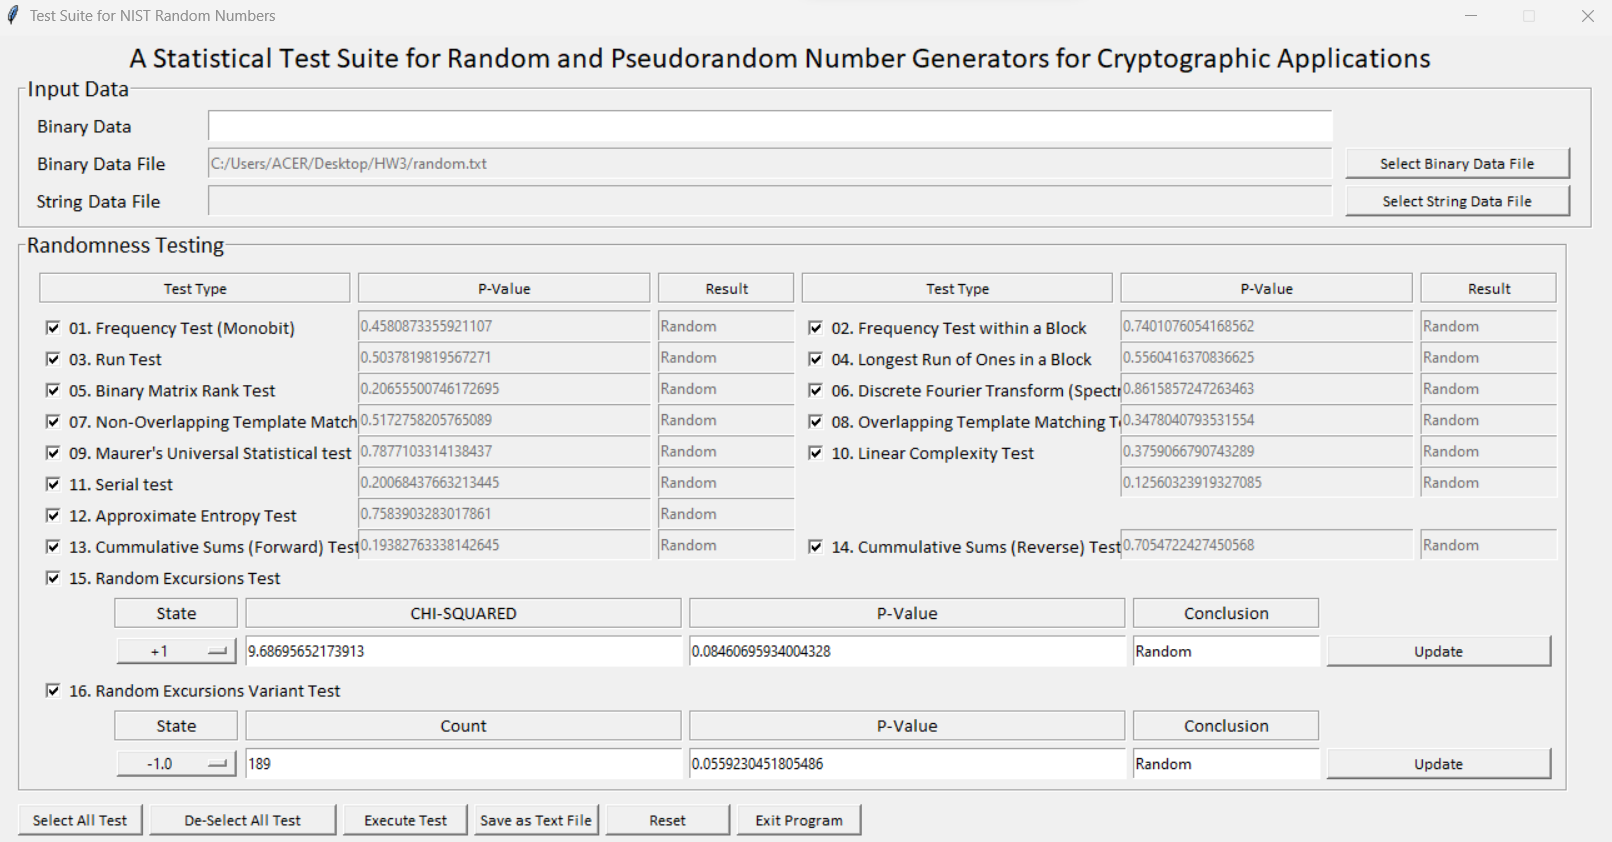
\includegraphics[scale=0.4]{hw03-1884749}
\\\\\\
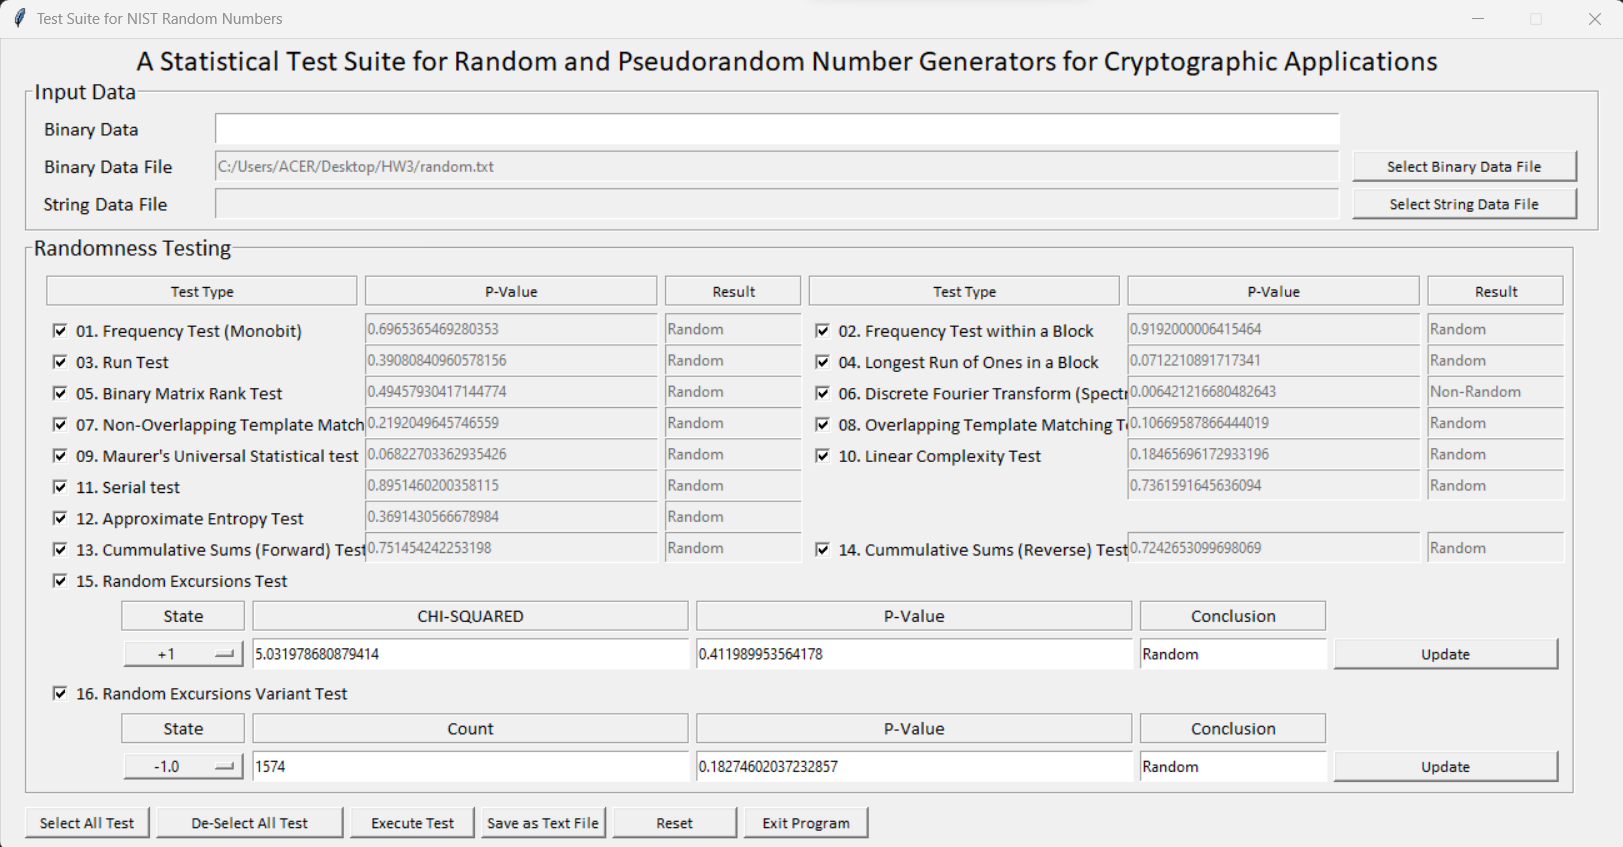
\includegraphics[scale=0.4]{hw03-1884749-1}
\\
In the first image we used a CSPRGN and passed all tests, we can see the result "random" in all tests, very good result in the monobit test(number of ones and numbers of zeros). The random library used in the second image not passed all the tests, in discrete fourier transformation we have not-random, and have worst results in all tests respect to CSPRNG. But these tests doesn't guarantee that one generator is better than another, in fact random library have passed nearly all tests, in the practice we have not much difference with our implementation of CSPRNG. But like we said in the first section a very good attacker can find some kind of patter in the generator of python, is always better to use implementation of CSPRNG because are based on more strong analysis. Analyzing the random library of python we will find that the random number generator has a fixed width, on a 64 bit system the generator can only generate \begin{math}2^{64}\end{math} different unique sequences, you can not therefore use it for simulations which requires a very large number of random trials. Also like we do in implementation we must guarantee that the range used from the generator have same number of odd and even numbers because otherwise we can construct some method for predict the next bit in the sequence (Ex. our range in random library script is (3,20000) that contain same odd and even number).
\end{document}